%!TEX root = ../RASD/main.tex

\subsection{Scenarios}
\label{sec:scenarios}
This section describes the most common scenarios of the \emph{system-to-be} highlighting all the interactions between the \emph{\nameref{def:user}} and the system.

% Sign Up
\subsubsection{User Sign-up} 
\label{ssub:sign_up_scenario}
\paragraph{Scenario} 
Alice is tired of calling a taxi by phone. So she decides to download a new app called \emph{MyTaxiService}.
Once the download is completed she opens the app and signs-up providing her email, name, surname, password, date of birth and ID.
% Table
\import{../tables/}{registrationtable.tex}

% Sequence diagram
\newpage
\vfill
\begin{figure}
\caption{Sequence Diagram}
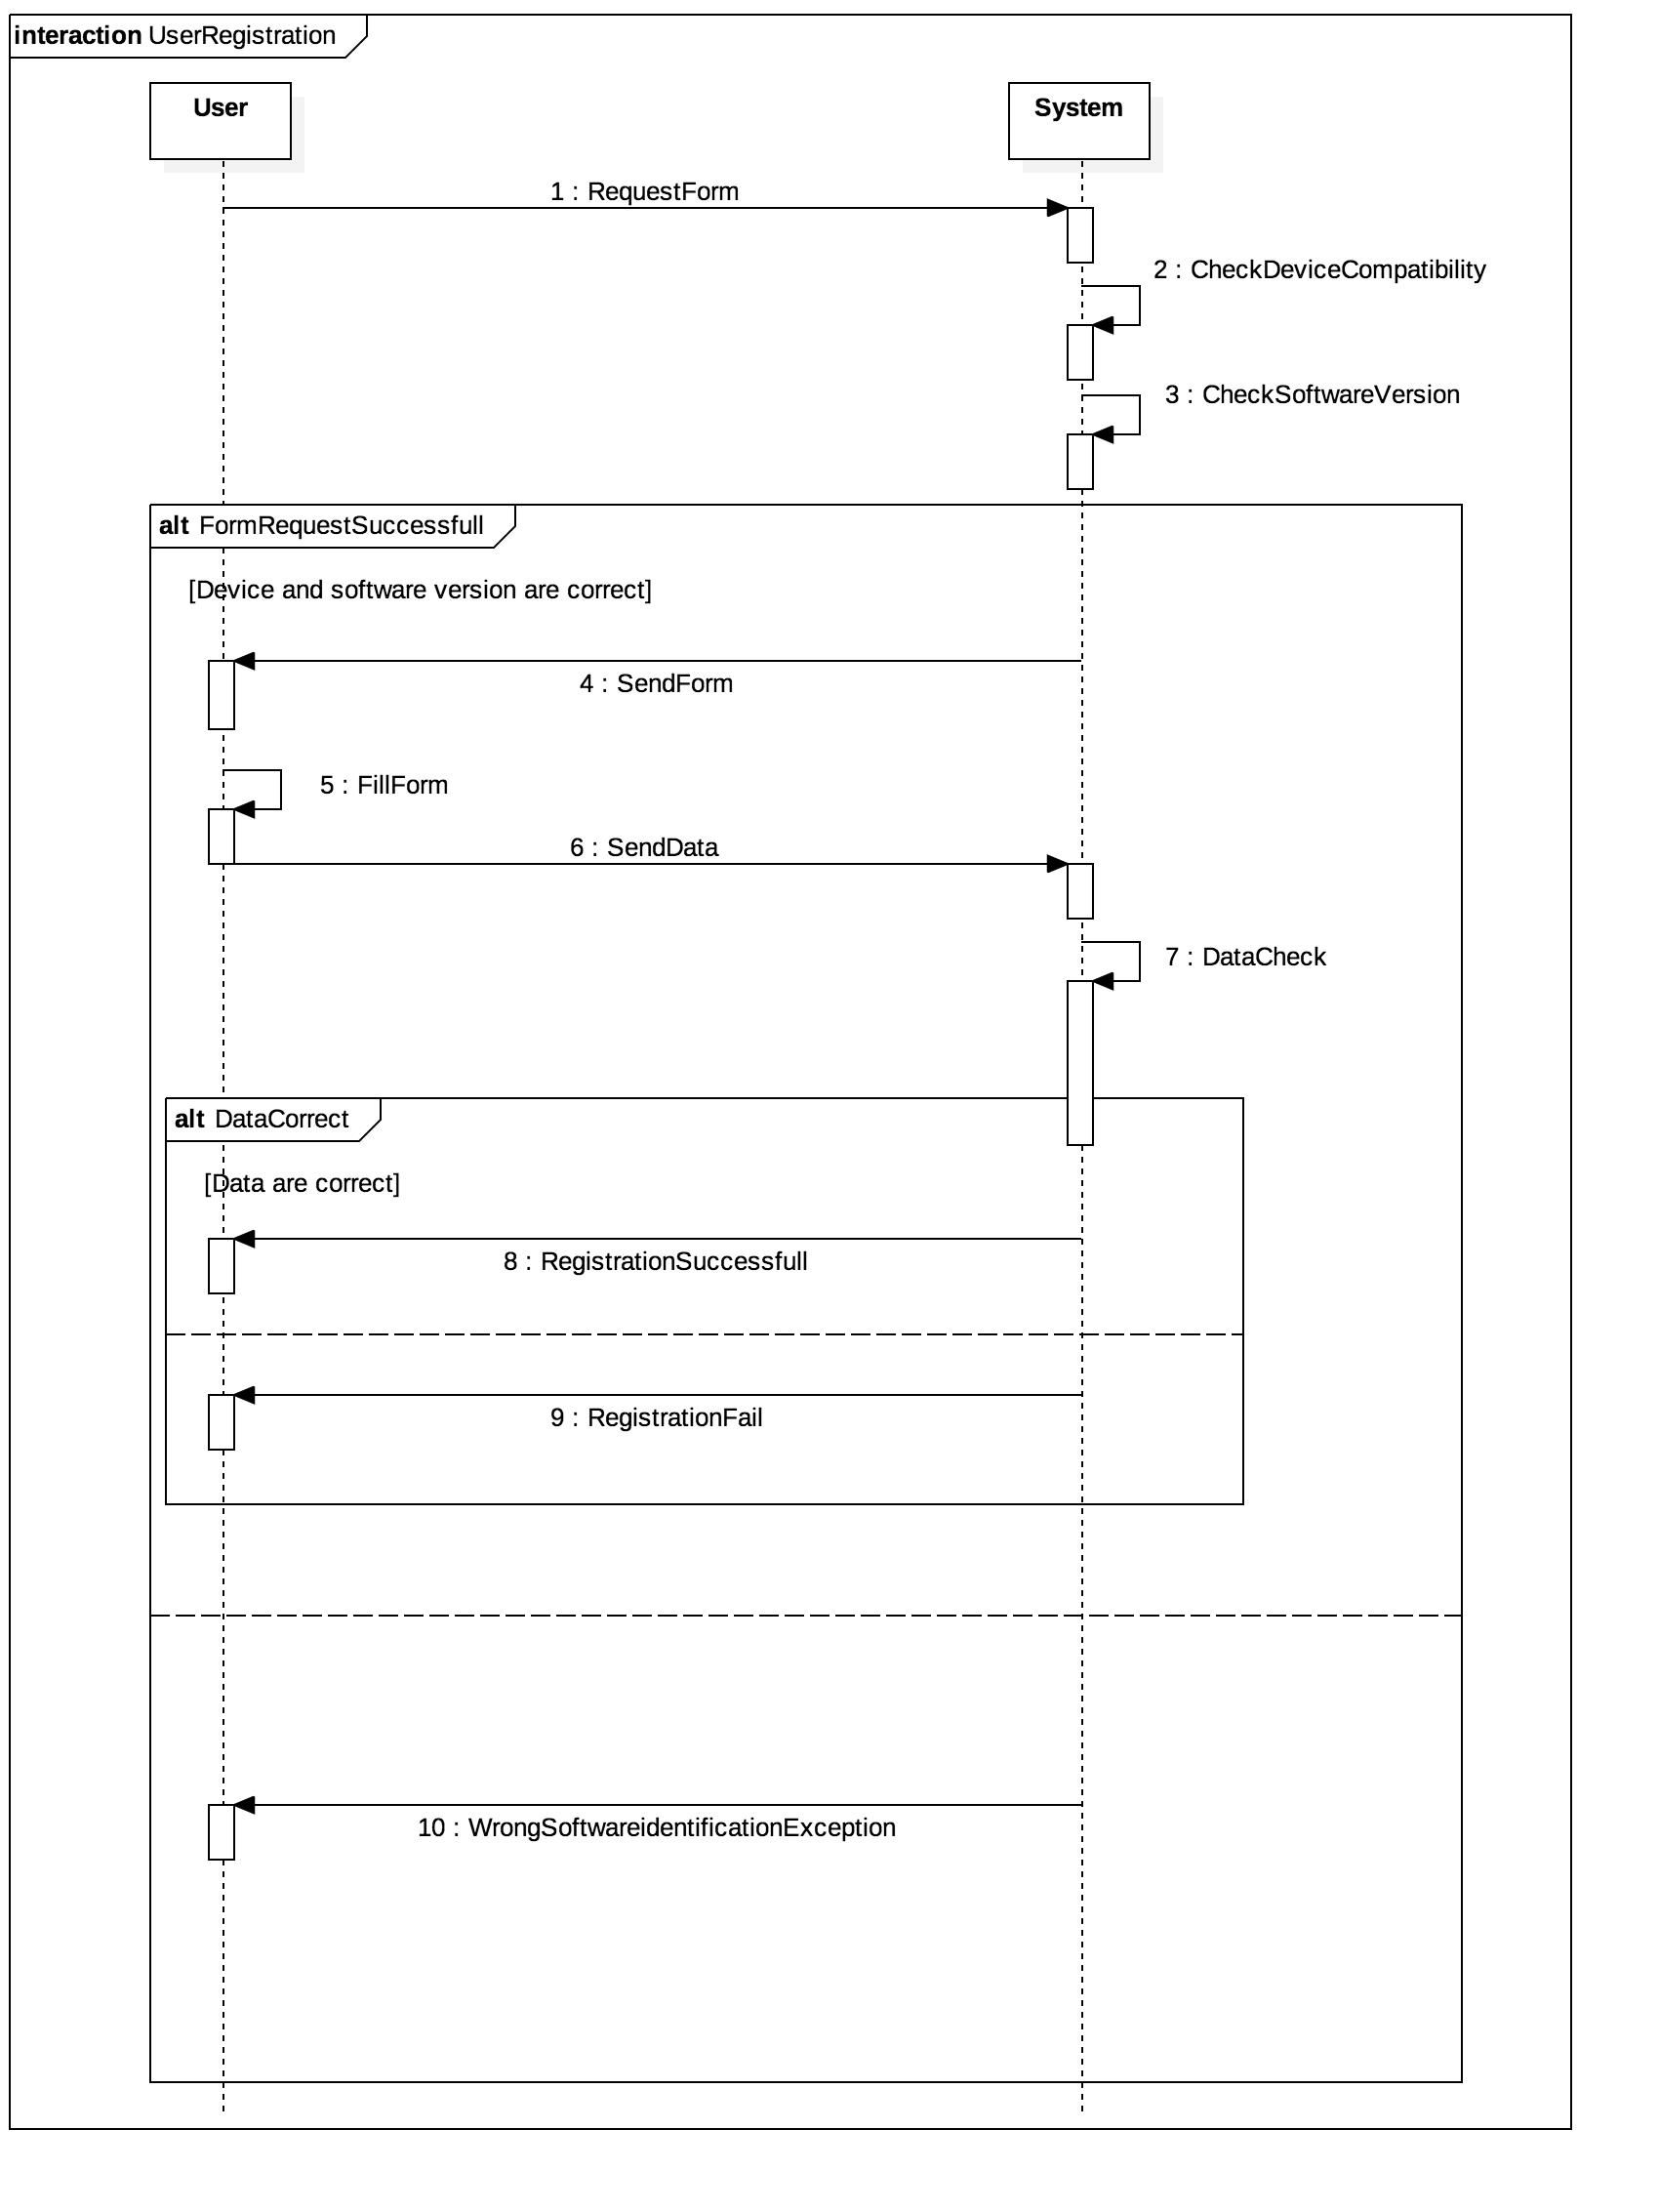
\includegraphics[width=\textwidth]{sequence-diagrams/Collaboration1__Interaction1__UserRegistration_1}
\centering
\end{figure}
\vfill
\clearpage


% Log in
\subsubsection{User Log in} 
\label{ssub:login_scenario}
\paragraph{Scenario} \hfill \\
Bob is a registered user. Bob wants to book a taxi, he opens the mobile app, he provides his email and his password and after the verification he can access the service.
% Table
\import{../tables/}{logintable.tex}
% Sequence diagram
\newpage
\vfill
\begin{figure}
\caption{Sequence Diagram}
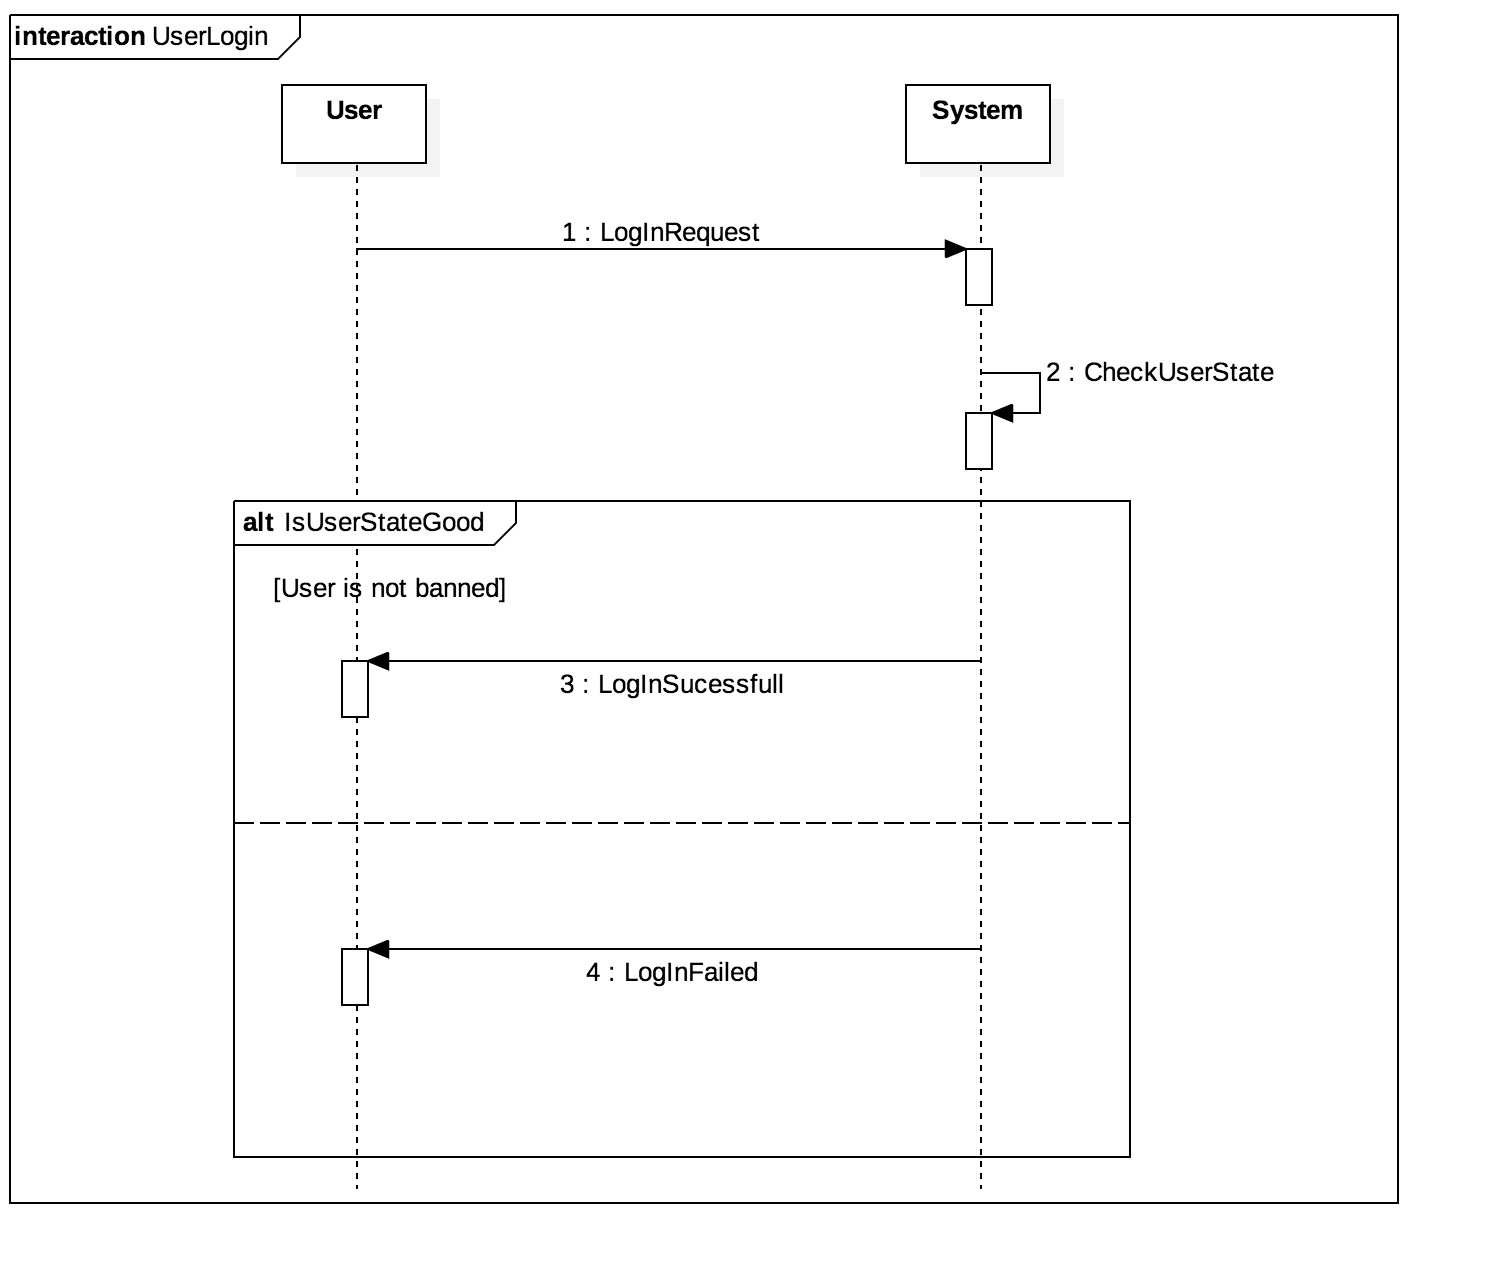
\includegraphics[width=\textwidth]{sequence-diagrams/Collaboration2__Interaction1__UserLogin_2}
\centering
\end{figure}
\vfill
\clearpage

% Modify data
\subsubsection{Modify Data} 
\label{ssub:modify_scenario}
\paragraph{Scenario} \hfill \\
Alice is logged in. She wants to change some data she entered wrong. 
% Table
\import{../tables/}{modifydatatable.tex}
% Sequence diagram
\newpage
\vfill
\begin{figure}
\caption{Sequence Diagram}
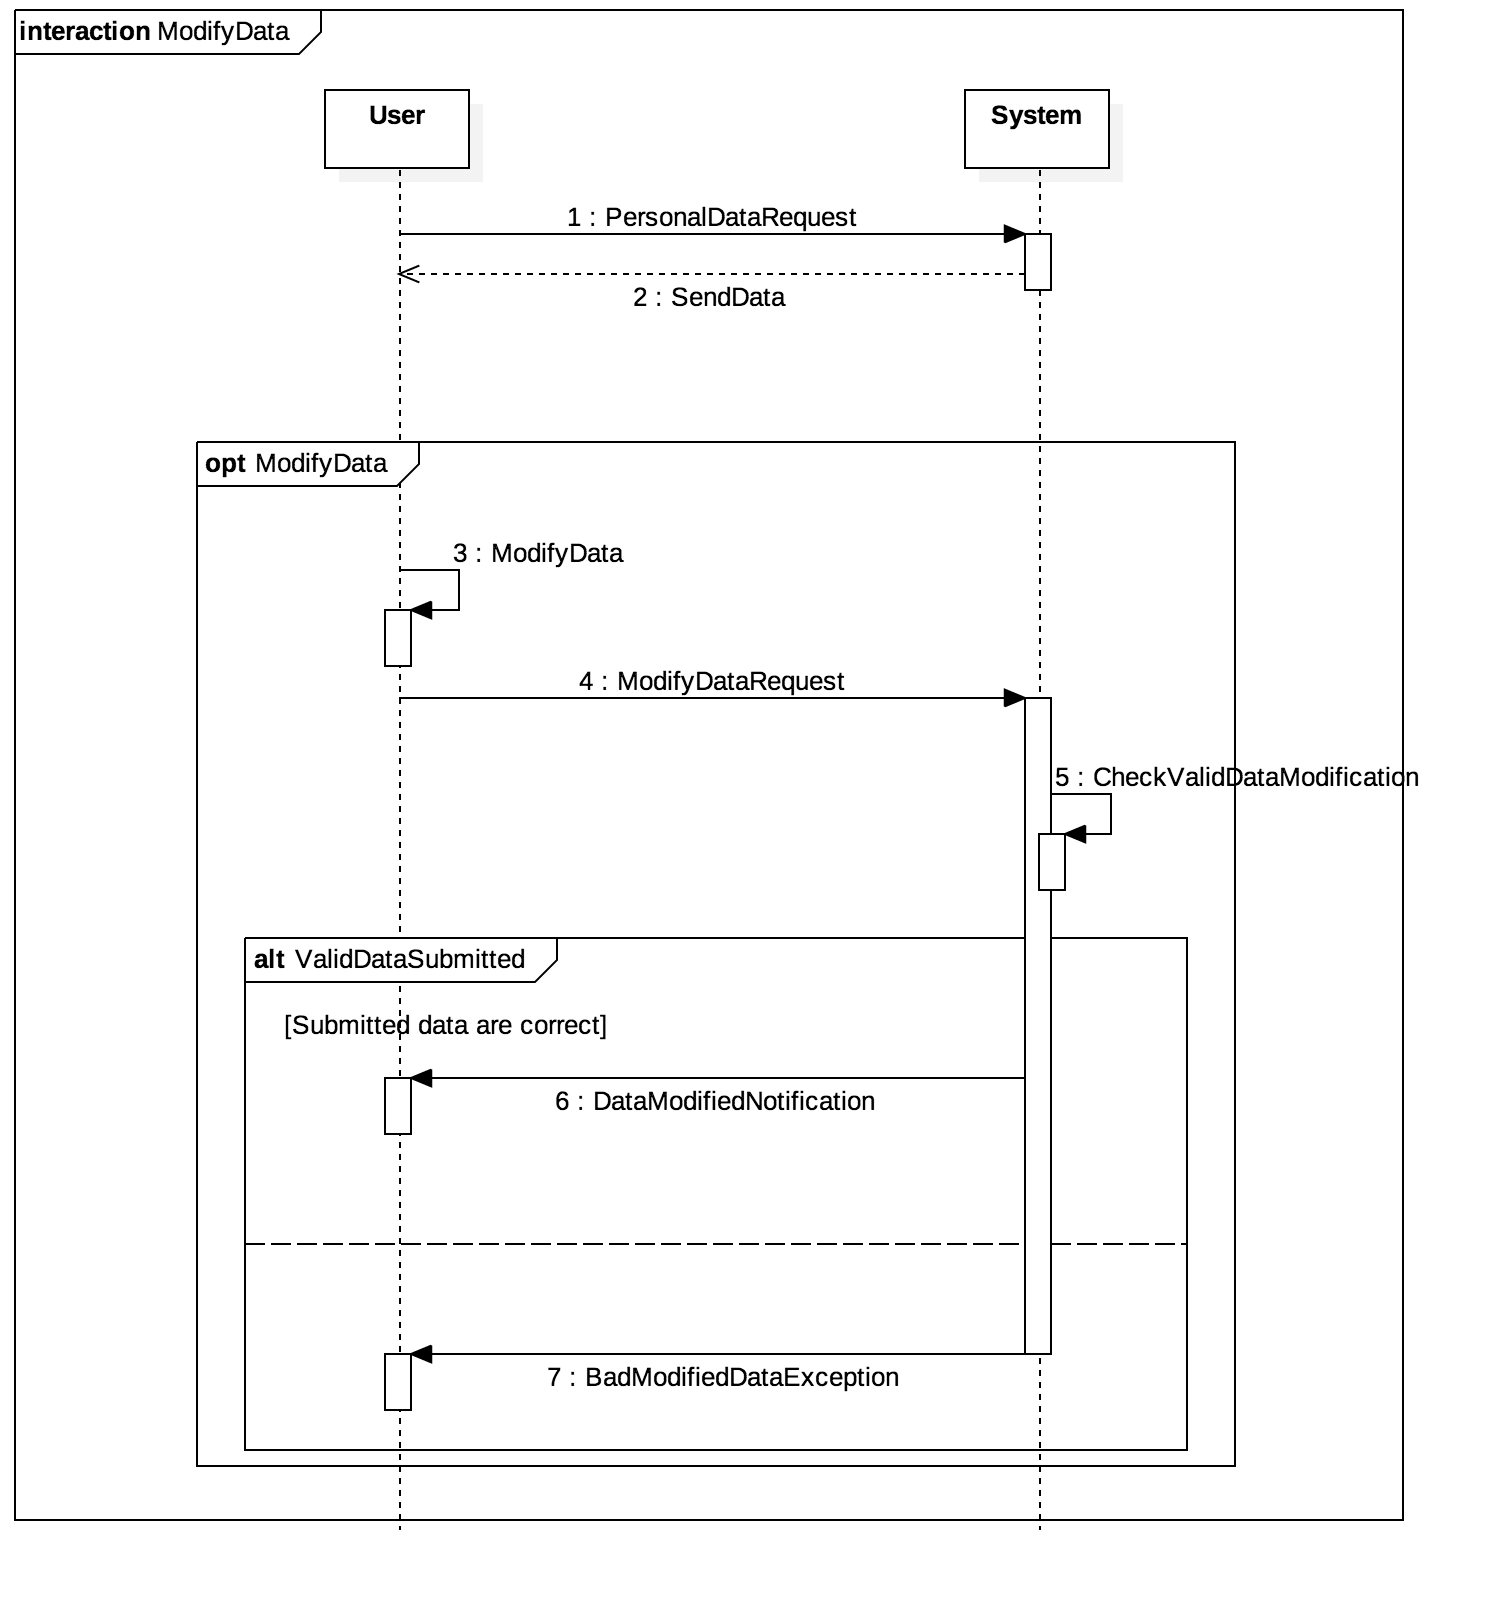
\includegraphics[width=\textwidth]{sequence-diagrams/Collaboration8__Interaction1__ModifyData_7}
\centering
\end{figure}
\vfill
\clearpage

% Taxi request
\subsubsection{Taxi Request} 
\label{ssub:taxirequest_scenario}
\paragraph{Scenario} \hfill \\
Alice is logged in. She wants to book a taxi. She opens the app, she fills all the fields, she asks for a taxi and waits for the response.\\
Bob is a taxi driver, he is now free.\\
Bob receives a ride request and decide whether to accept it or not.
% Table
\import{../tables/}{userbooktaxitable.tex}
% Sequence diagram
\newpage
\vfill
\begin{figure}
\caption{Sequence Diagram}
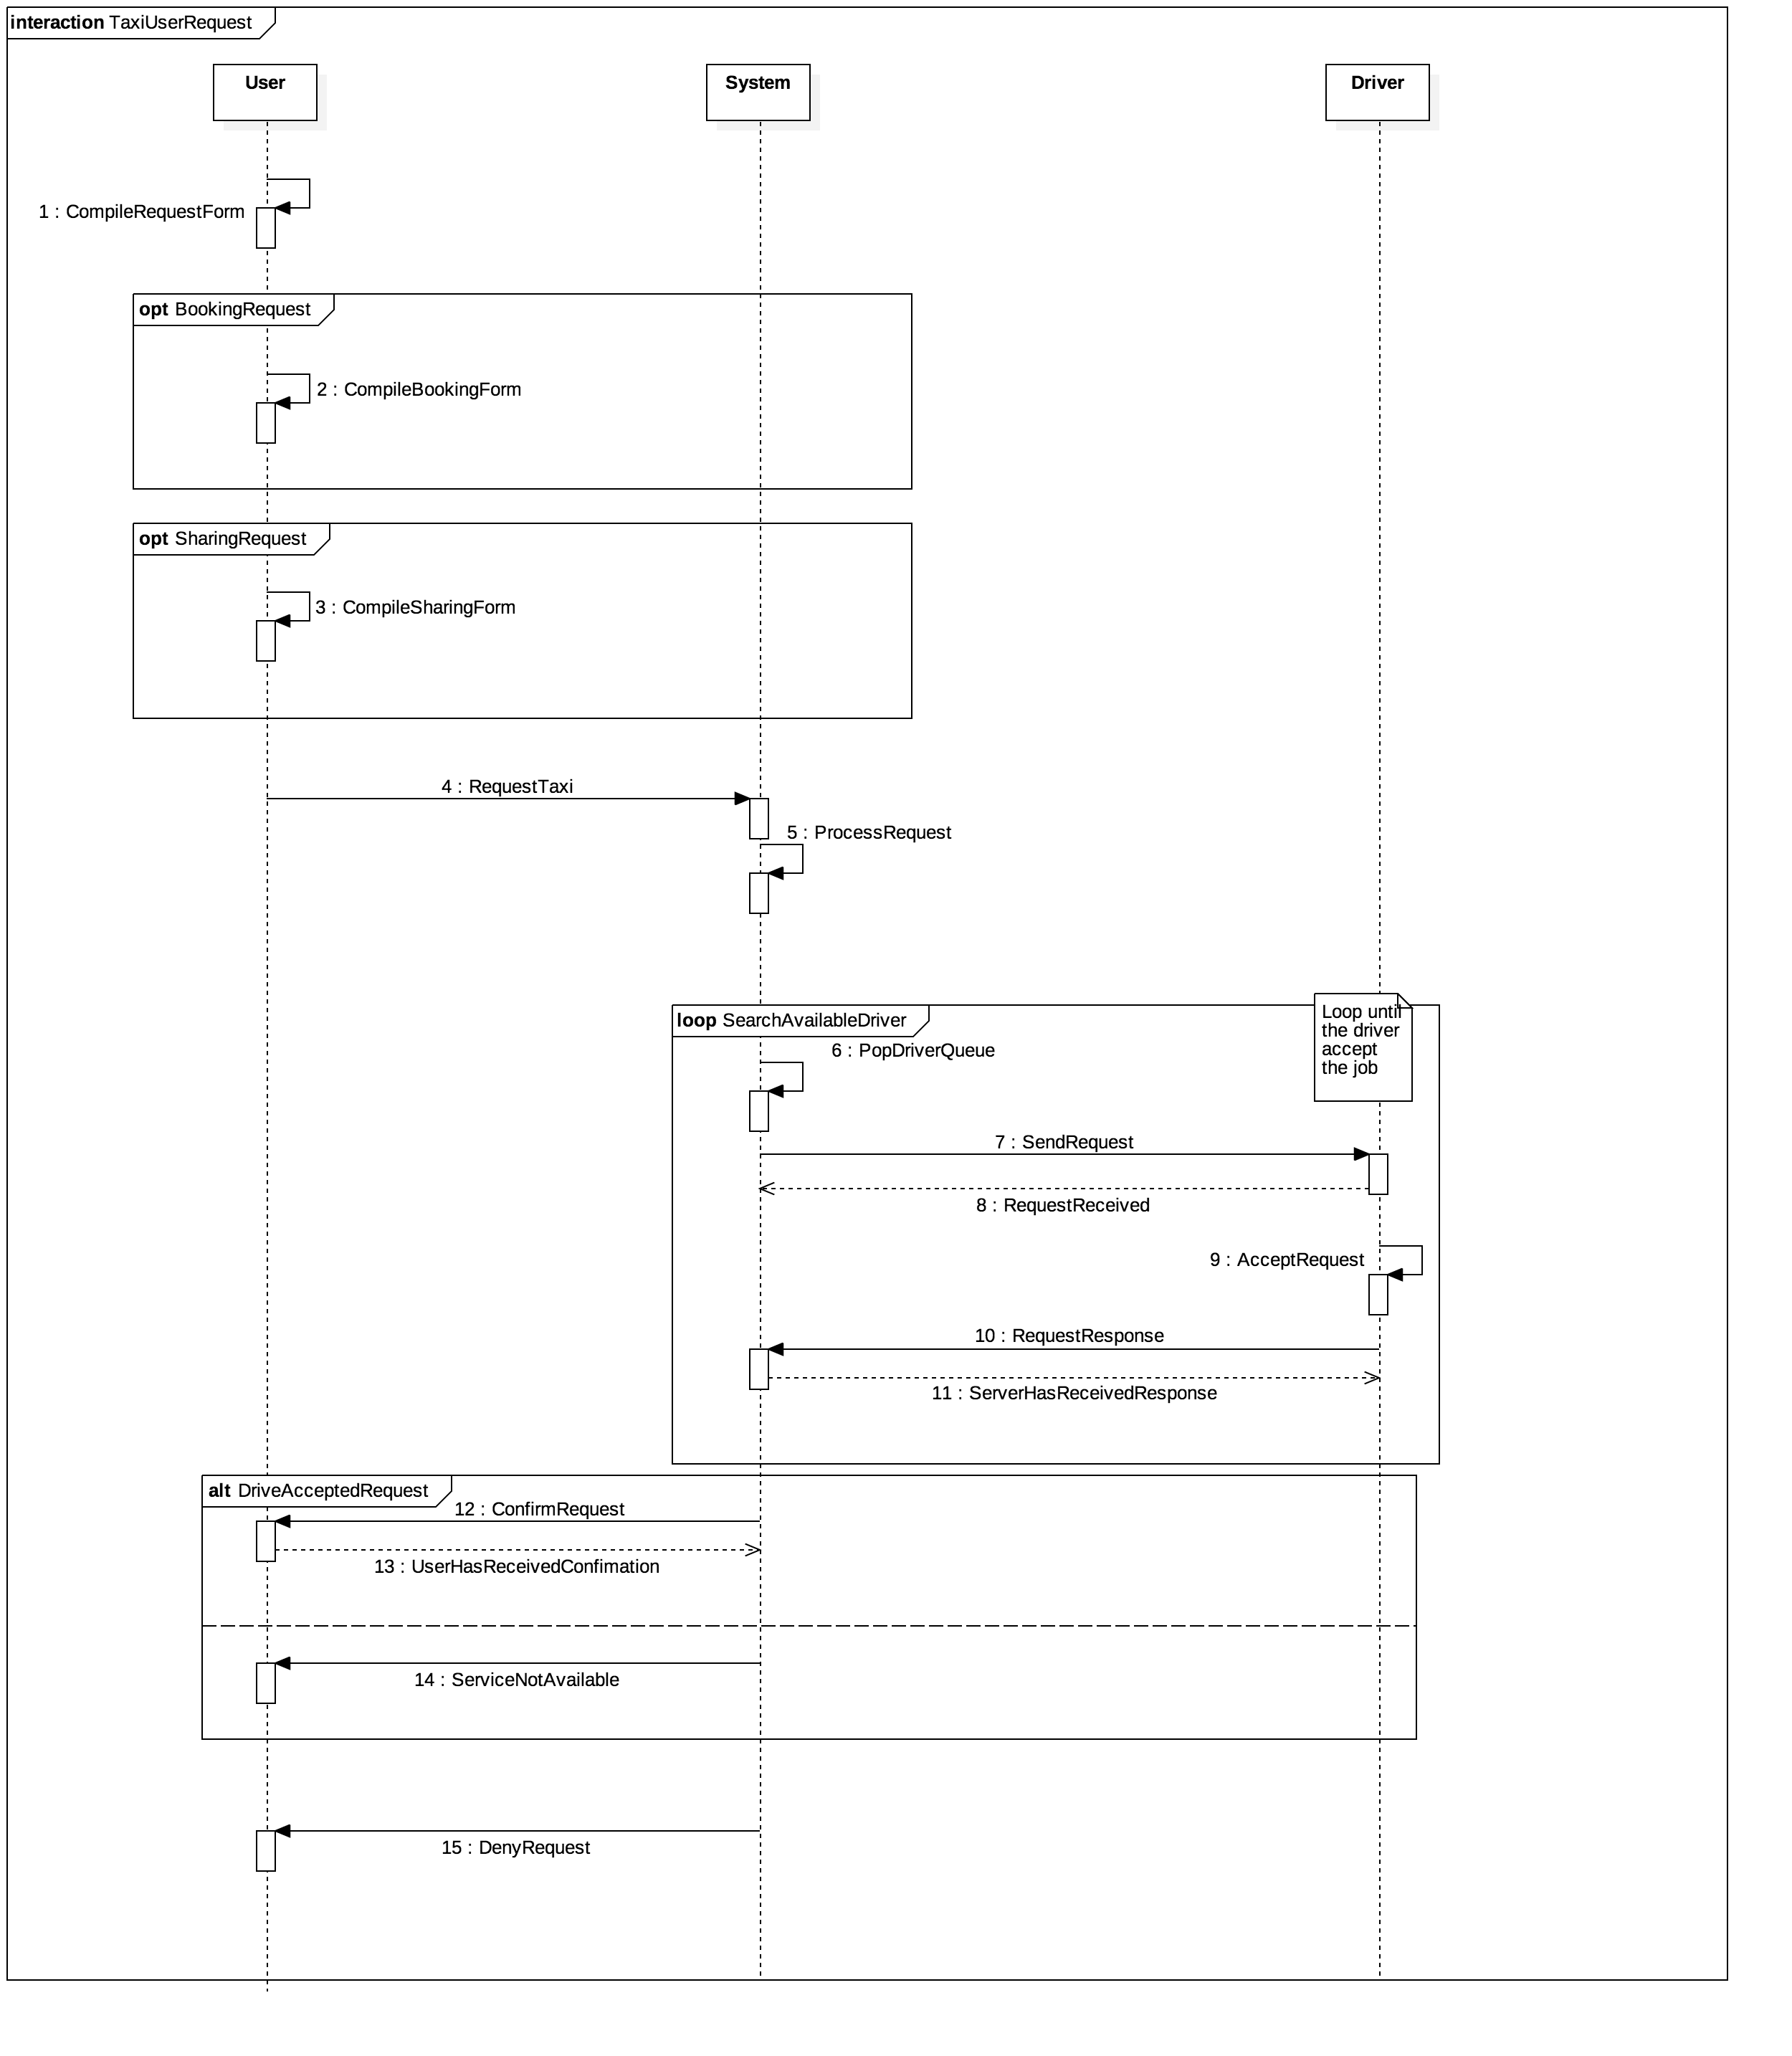
\includegraphics[width=\textwidth]{sequence-diagrams/Collaboration3__Interaction1__TaxiUserRequest_3}
\centering
\end{figure}
\vfill
\clearpage

% Taxi driver registration
\subsubsection{Taxi Driver Registration} 
\label{ssub:taxidriverregisration_scenario}
\paragraph{Scenario} \hfill \\
Bob, a support operator receives a new mail from Alice, a taxi driver who wants to join the service. Bob checks the validity of the license and reply to Bob.
% Table
\import{../tables/}{registerlicensetable.tex}
% Sequence diagram
\newpage
\vfill
\begin{figure}
\caption{Sequence Diagram}
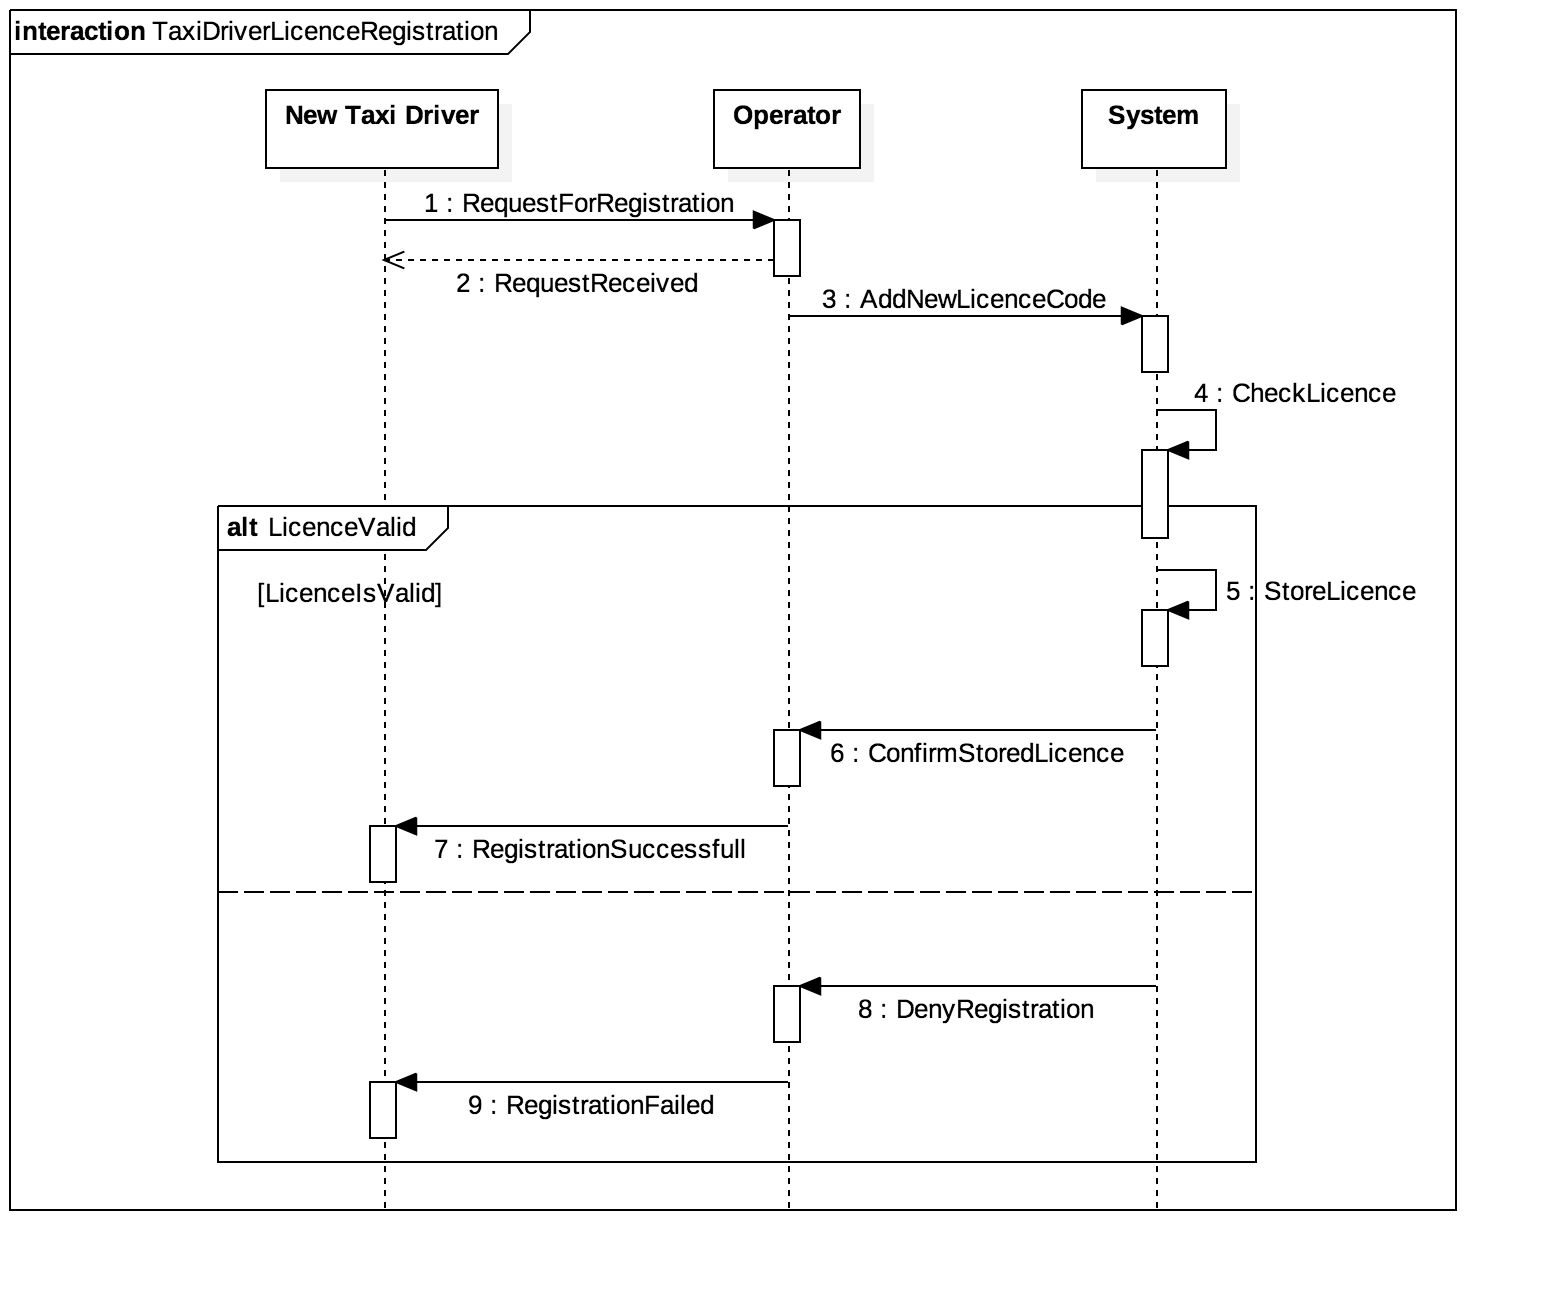
\includegraphics[width=\textwidth]{sequence-diagrams/Collaboration5__Interaction1__TaxiDriverLicenceRegistration_4}
\centering
\end{figure}
\vfill
\clearpage

% Delete request
\subsubsection{Delete Request} 
\label{ssub:deleterequest_scenario}
\paragraph{Scenario} \hfill \\
Bob asked for a taxi 2 minutes ago. Bob finds out he does not need a taxi ride anymore. Bob tries to delete his ride request. The system decides if the delete request is on time and legit.
% Table
\import{../tables/}{deleterequest.tex}
% Sequence diagram
\newpage
\vfill
\begin{figure}
\caption{Sequence Diagram}
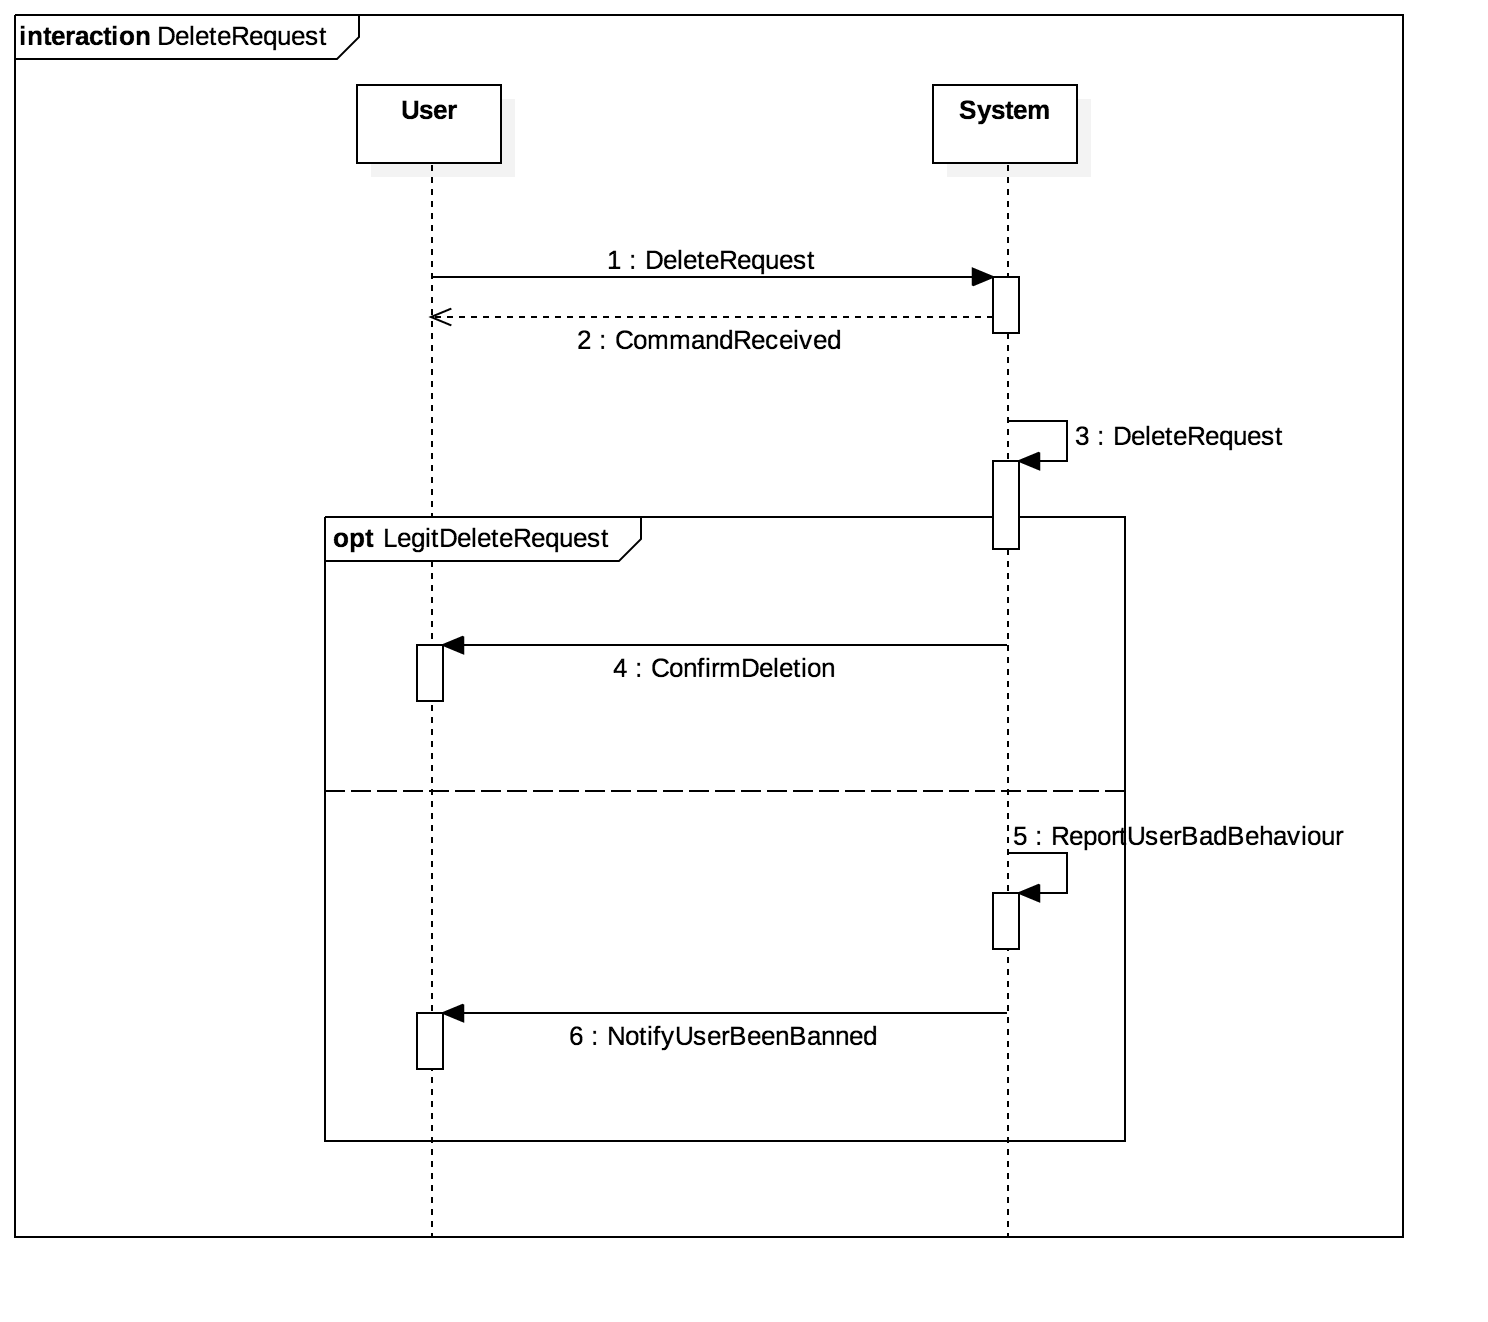
\includegraphics[width=\textwidth]{sequence-diagrams/Collaboration6__Interaction1__DeleteRequest_5}
\centering
\end{figure}
\vfill
\clearpage

% Report problem
\subsubsection{Report Problem} 
\label{ssub:reportproblem_scenario}
\paragraph{Scenario} \hfill \\
Bob is a taxi driver. Bob is riding his cab while a incident occurs and he will have to wait at least 30 minutes. Bob report the incident to the system using the app.
% Table
\import{../tables/}{reportproblemtable.tex}
% Sequence diagram
\newpage
\vfill
\begin{figure}
\caption{Sequence Diagram}
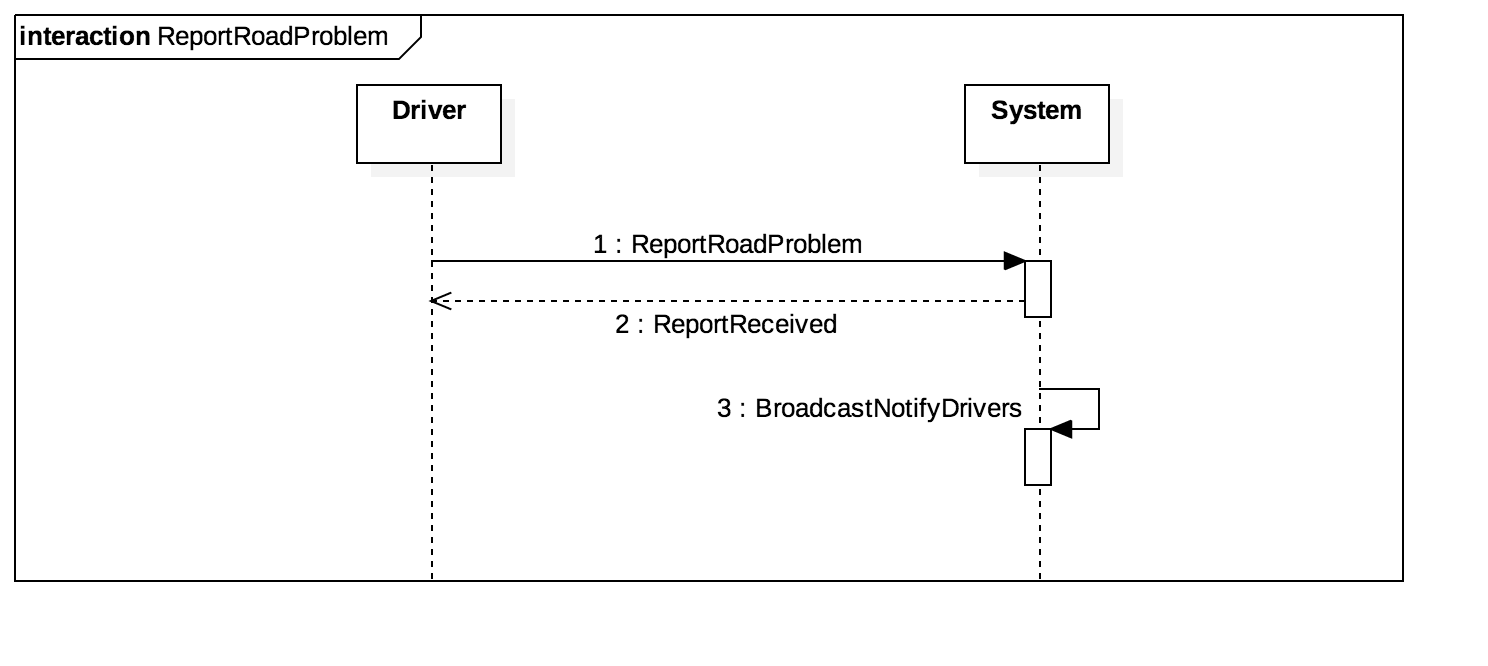
\includegraphics[width=\textwidth]{sequence-diagrams/Collaboration7__Interaction1__ReportRoadProblem_6}
\centering
\end{figure}
\vfill
\clearpage

% Report problem
\subsubsection{Ride Sharing} 
\label{ssub:ridesharing_scenario}
\paragraph{Scenario} \hfill \\
Bob wants to cut the price of the taxi ride he is booking. He decides to enable the sharing option on the app.\\
Alice wants to cut the price too.\\
She decides to enable the sharing option on the app and if their paths are admissible, the will share the same ride.
% Sequence diagram

\begin{figure}[h!t]
\caption{Sequence Diagram}
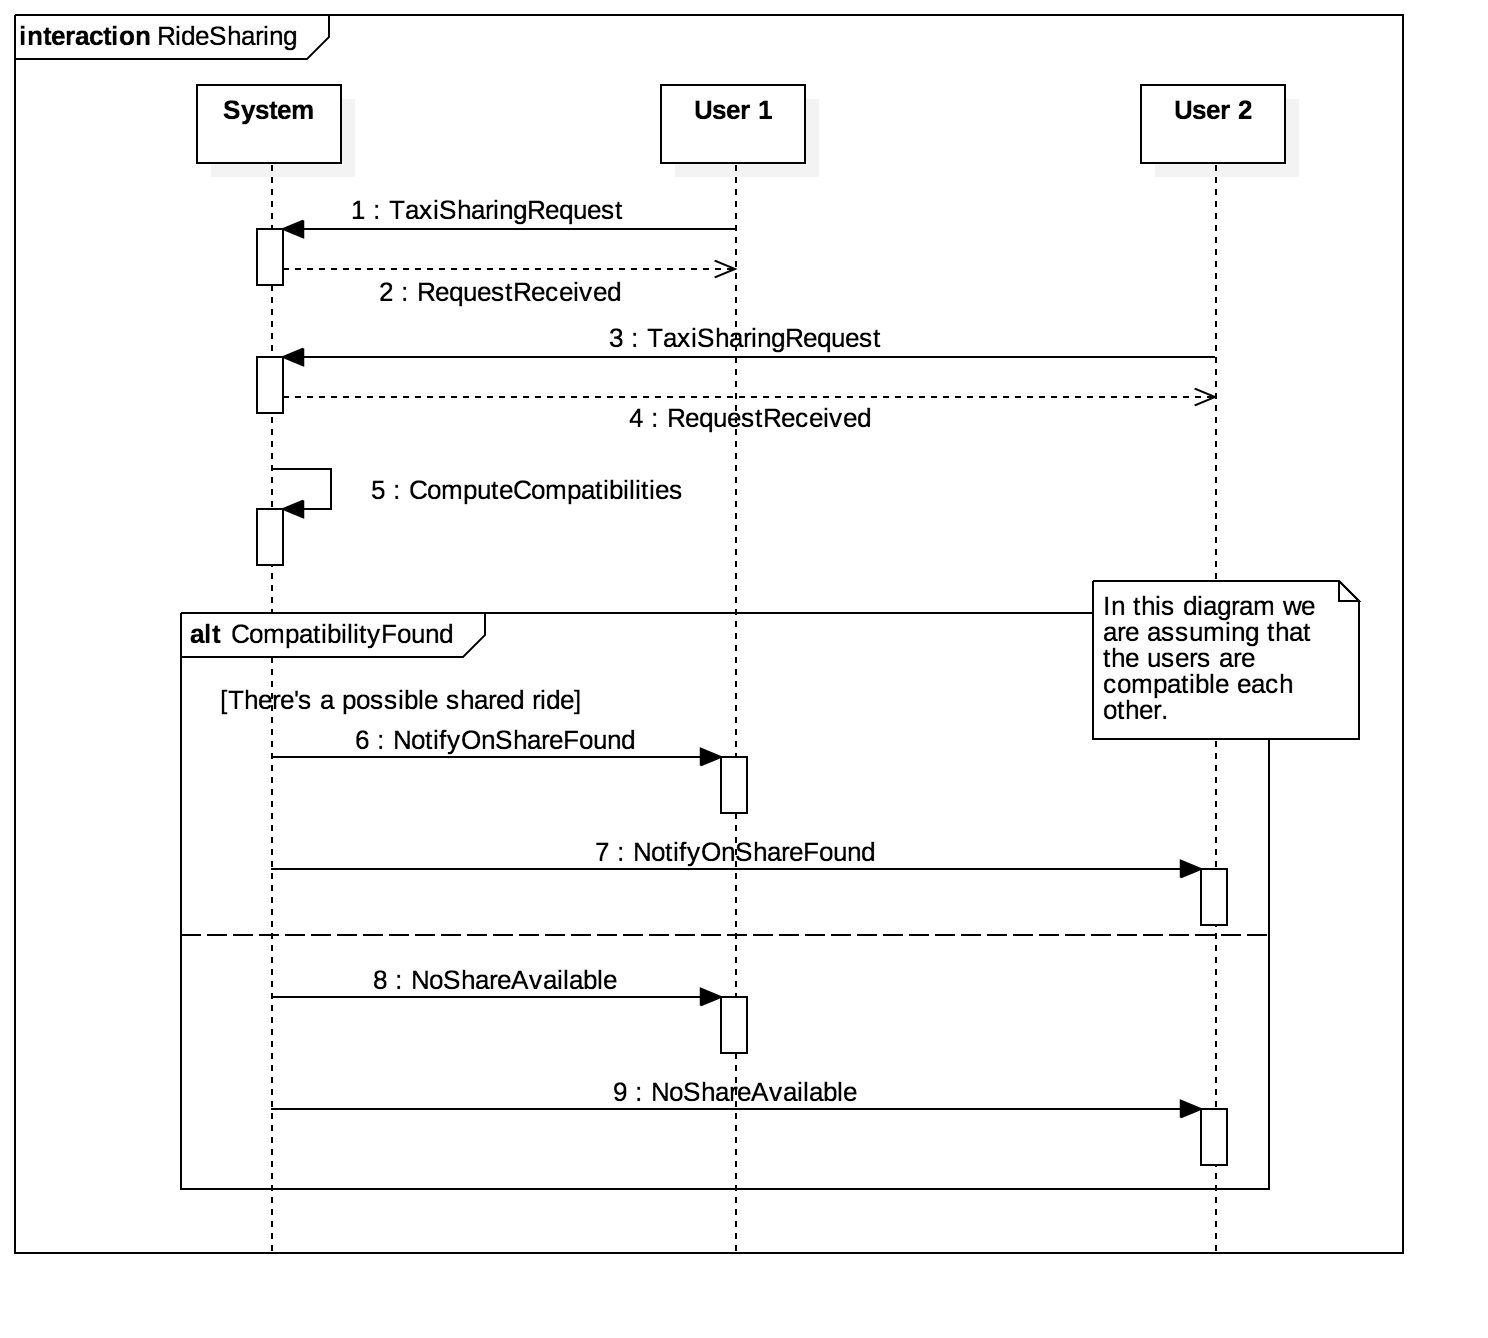
\includegraphics[width=\textwidth]{sequence-diagrams/Collaboration9__Interaction1__RideSharing_12}
\centering
\end{figure}

\newpage
\subsection{Class Diagram} 
\begin{figure}[h!t]
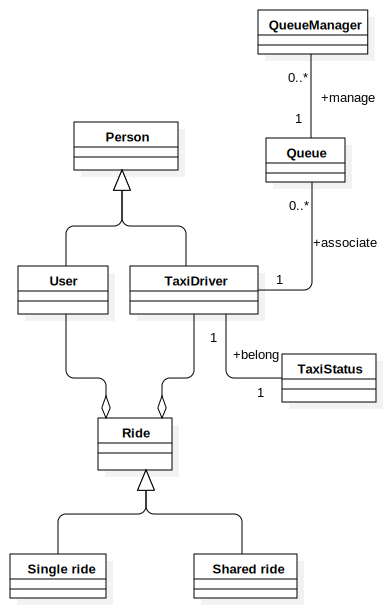
\includegraphics[width=\textwidth]{class-diagrams/ClassDiagram1}
\centering
\end{figure}
\newpage

\subsection{State Charts} 
Here are presented the state charts of the main objects of the \emph{system-to-be}

\begin{figure}[h!]
\caption{User State Chart}
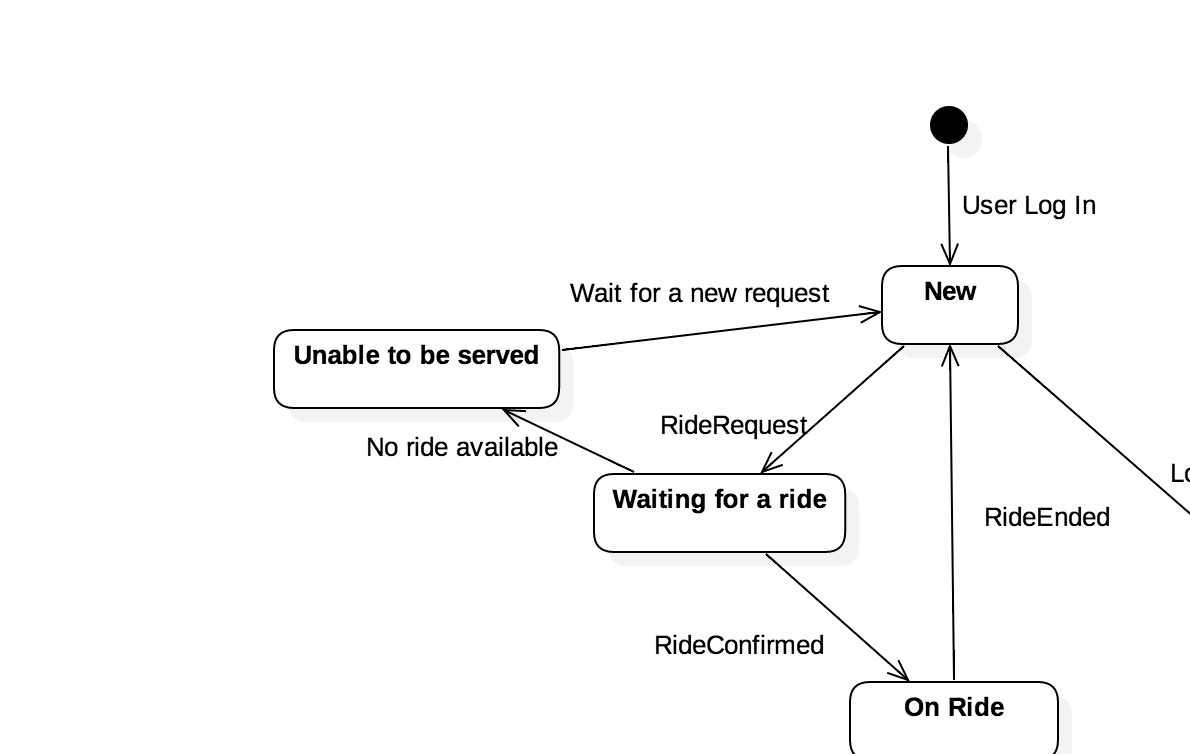
\includegraphics[width=\textwidth]{state-charts/StateMachine2__UserStateChart_10}
\centering
\end{figure}

% Ride
\newpage
\vfill
\begin{figure}
\caption{Ride State Chart}
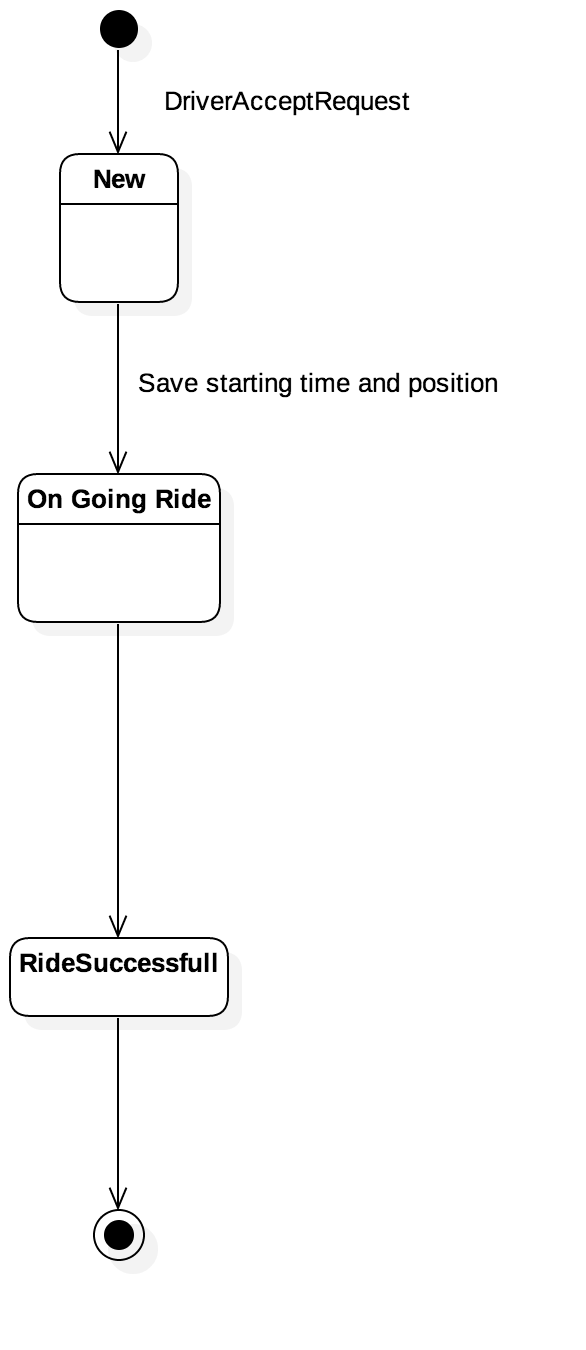
\includegraphics[width=\textwidth]{state-charts/StateMachine1__RideStateChart_9}
\centering
\end{figure}
\vfill
\clearpage


% Driver
\newpage
\vfill
\begin{figure}
\caption{Driver State Chart}
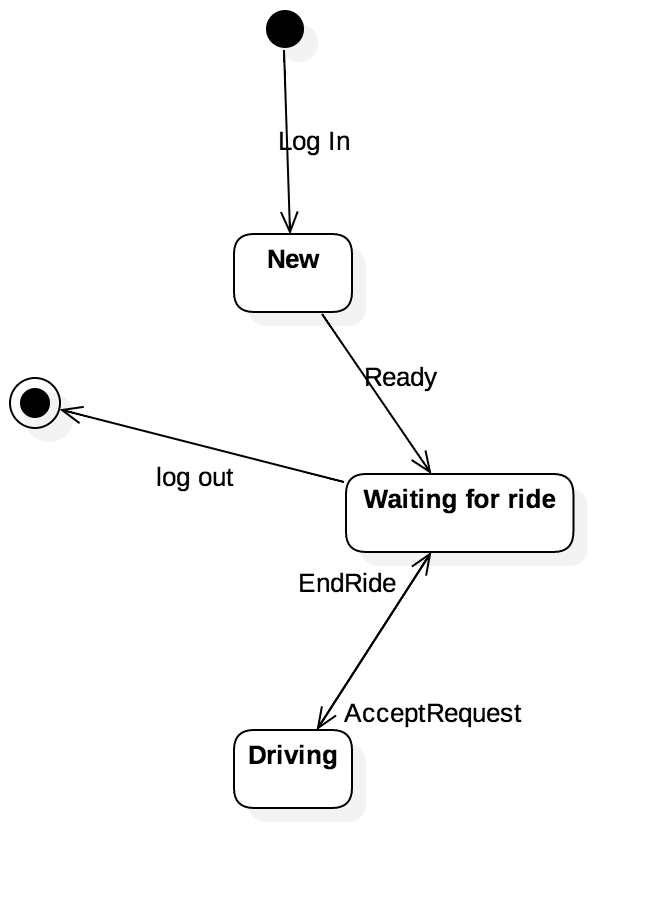
\includegraphics[width=\textwidth]{state-charts/StateMachine3__DriverStateChart_11}
\centering
\end{figure}
\vfill
\clearpage
